\chapter{Bioinformatyka w praktyce}

%\subsection{Farmaceutyka}
%\subsection{Kryminalistyka}
%\subsection{Sądownictwo}
%\subsection{Rolnictwo}
%\subsection{Archeologia}

%\section{Bioinformatyka w ujęciu algorytmicznym}
%\subsection{Bazy danych}
%\subsection{big data}
%\subsection{uczenie maszynowe}
%\subsection{metody optymalizacji}
%\subsection{teoria grafów}

\section{Problemy bioinformatyki}
\info{Y źródło\\}
Bioinformatyka, jak każda dziedzina naukowa boryka się z pewnymi problemami. Problem dotyczący baz danych polega na tym, że wiele baz powstaje i często potem nic się z nimi nie dzieje. Z każdym dniem poznajemy tysiące nowych sekwencji, które są deponowane w cyfrowych przechowalniach. Te podstawowe bazy są utrzymywane i z powodzeniem wykorzystywane do naukowych doświadczeń, jednakże problemem są bazy wtórne, bazujące na wynikach z wcześniejszych, podstawowych eksperymentów. Gromadzą one najczęściej zbiór informacji pochodzący z różnych miejsc i często są one po stosunkowo niedługim czasie nieaktualne.

Projekty bioinformatyczne często zostają zakończone opracowaniem bazy danych, po czym finansowanie projektu kończy się, projekt nie jest kontynuowany.
Jako, że mamy do czynienia z danymi biologicznymi oznacza to, że eksperymenty zazwyczaj obarczone są jakimś ryzykiem błędu. Niejednokrotnie zdarza się, że do bazy pierwotnej są wprowadzane modyfikacje, które nie zostają już uwzględnione w późniejszych bazach wtórnych. Błędy te propagują się na następne projekty. W~przypadku zakończenia projektu bazy wtórnej, pomimo aktualizacji danych pierwotnych, na których się opierała, informacje wtórne nie zostają już zmienione. Jest to dość poważny problem z jakim obecnie świat bioinformatyki boryka się.

Wspomniane zbiory danych często są ogromne. Sekwencja przykładowego genomu człowieka zajmuje ponad 3GB, natomiast opis samego eksperymentu sekwencjonowania może zająć nawet kilkaset gigabajtów. Pojawiający się problem jest natury technicznej - chodzi o sposób przechowywania danych. Okazuje się, że często bardziej opłaca się laboratorium ponownie przeprowadzić eksperyment sekwencjonowania, niż przechowywać wyniki doświadczeń na dyskach, gdyż jest to zbyt kosztowne. 

Kolejnym problemem jest mnogość standardów. Często gdy jest jakiś problem, rozwiązanie projektowane jest od podstaw. Takie podejście skutkuje tym, że dla pojedynczego zadania, mamy kilkanaście bądź kilkadziesiąt różnych metod, które nie koniecznie są ze sobą kompatybilne. Jednym z głównych problemów, z jakim zmagają się biolodzy przy analizie danych jest to, że wyjście z jednego programu nie jest kompatybilne z wejściem drugiego programu, który potrzebują aktualnie wykorzystać. Próby rozwiązania takiego kłopotu skutkują często zdefiniowaniem kolejnego standardu, co może jeszcze bardziej skomplikować sytuację jeśli nowy sposób się nie zostanie przyjęty przez większe grono naukowców.


%-niekontynuowane projekty \\
%-dane bazują na eksperymentach, błędy propagujące się \\
%-wiele różnych standardów, niekompatybilne \\
%-nieinformatyczni biolodzy \\
%-sposoby finansowania nauki \\

\section{Centralny dogmat bioinformatyki}
Podstawowym założeniem w bioinformatyce jest następująca zależność:
Informacja, która jest zawarta w sekwencji nukleotydowej bezpośrednio przekłada się na strukturę przestrzenną białek i innych cząsteczek, które są w genomie zakodowane. Dzięki strukturze przestrzennej, białka mogą na siebie bezpośrednio oddziaływać, co oznacza że pełnią one pewne funkcje biochemiczne. Funkcją biochemiczną może być np. reakcja w którą wchodzi dane białko łącząc się z inną substancją. Efekt końcowy oddziaływań zbioru wybranych białek obserwujemy w postaci np. wyglądu zewnętrznego, zachowania, funkcjonowania organizmu.

Informacje sekwencyjne jesteśmy w stanie eksperymentalnie pozyskać bardzo łatwo. Trudniej jest określić struktury przestrzenne i funkcje biochemiczne jakie pełnią.
Obecnie nacisk jest wywierany na ustalenie procesu w jaki sposób na podstawie sekwencji możemy określić strukturę przestrzenną bądź później, funkcję danego związku chemicznego.
Z samej obserwacji fenotypu nic nie wynosimy. Dążymy do tego aby dowiedzieć się jakie konkretne białka odpowiadają za dany fenotyp. Chcemy posiąść kompletną wiedzę na temat funkcjonowania organizmu. Kryje się za tym znajomość wszystkich genów jakie mogą w tym organiźmie występować, odmian, mutacji i ch wzajemnych wpływów.

\begin{figure}[h]
	\centering
	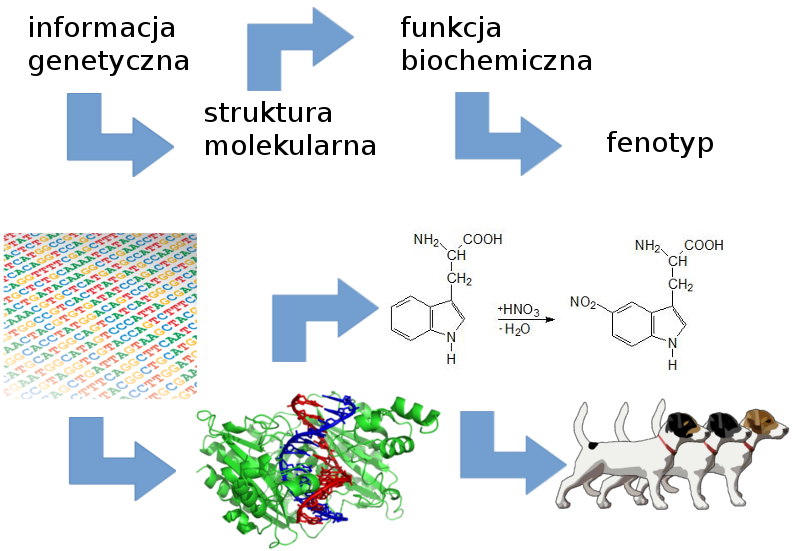
\includegraphics[width=0.9\textwidth]{img/centralny-dogmat.png}
	\caption{Centralny dogmat bioinformatyki}
	\vspace{-0.5cm}
	\caption*{\scriptsize Źródła: 
		\url{http://www.wikiwand.com/en/DNA},
		\url{http://igoscience.com/dna-sequence-genetic-code/} \\
		\url{https://commons.wikimedia.org/wiki/File\%3AReakcja\_ksantoproteinowa\_dla\_tryptofanu.jpg}, \\
		\url{https://www.russell-terrier.org/index.php/blog/56-maść-jrt-i-prt-w-praktyce-część-vi-fenotyp}
	}
	\label{img:centralny-dogmat}
\end{figure}

%-dna, rna, białko \\
%-informacja genetyczna \\
%-struktura molekularna \\
%-funkcja biochemiczna \\
%-fenotyp

%\section{Rozwój bioinformatyki}
%\subsection{wcześniej}
%\subsection{obecnie}
%\subsection{w przyszłości}

\section{Genom ogórka}
-sggw
